\section{Results}
\label{sec:results}



\subsection{Effect of semantic similarity}

Our primary contribution is the application and examination of using semantic similarity to compare node labels when comparing two trees, which would enable the use of tree distance on real world examples and not only on curated datasets. Of interest is how our datasets change with rising a semantic similarity limit ($\epsilon$). We expect that for each distance measure, that the distance between trees will increase with a rising $\epsilon$, as the semantic distance between two labels rises above $\epsilon$, nodes that were previously marked as matching (as the cosine similarity of their semantic embeddings was below $\epsilon$) become considered as needing a ``change'' operation. In Figures~\ref{fig:semsim-at1}~\ref{fig:semsim-at2}~and~\ref{fig:semsim-at1-2}, this is precisely the behavior we see. As described in Section~\ref{ssec:method-embeddings}, we use three pre-trained embeddings models in order to ensure that our results are not biased to a particular model. Each solid line is the mean value across the three models of the given distance, with the deviations above and below the mean value represented by the shaded areas.


\begin{figure}
    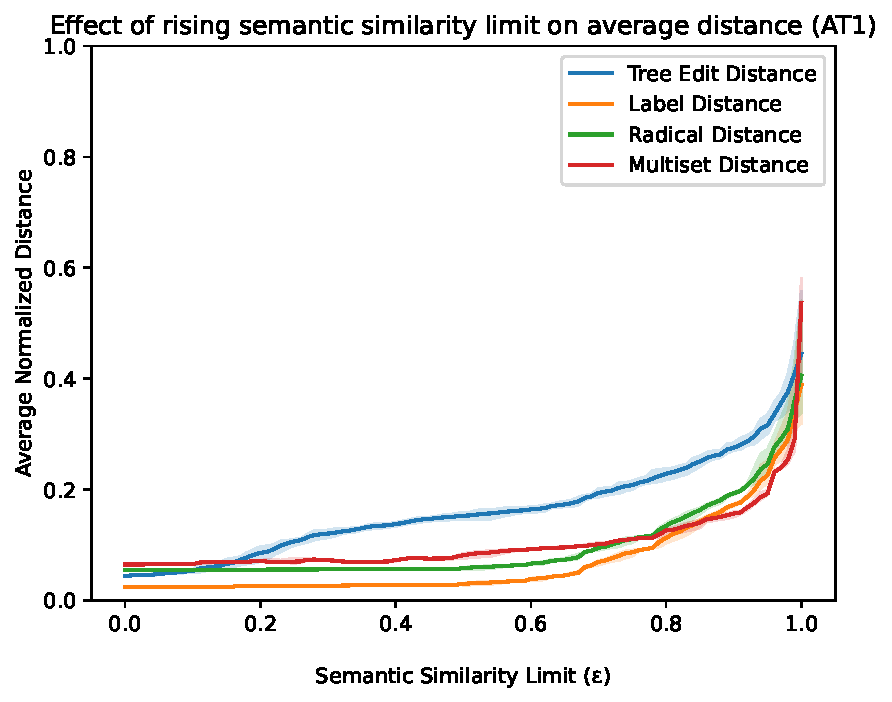
\includegraphics[width=\linewidth]{code/img/similaritylimits_at1_percentage.pdf}
    \caption{AT1 for semantic similarity limit ($\epsilon$) ranging from 0 to 1 with steps of 0.01}
    \label{fig:semsim-at1}
\end{figure}

In Figure~\ref{fig:semsim-at1}, we can see the normalized distance values for each of the distance measures. As described in Section~\ref{ssec:method-study-design}, \ATone\ consists of participants creating an attack tree from a written description (the attack tree shown in Figure~\ref{fig:tartgetAT}), which should result in idential (or nearly identical) tree. As we discussed in Section~\ref{ssec:method-analysis}, we expect to see distance measures that do not change with rising $\epsilon$. We can see that for LD, RD, and MSD, the normalized distances are all below 0.10, which show near identical trees for similarity limit ($\epsilon$) below ~0.7. Of note, TED shows an early increase in distance for similarity limit ~0.15 and then matches this later increase around 0.7 of the other three distance measures. As we show later in Table~\ref{tab:counterexamples}, this is likely be due to the order of nodes. Overall, this results suggest that a similarity limit ($\epsilon$) between 0.6 and 0.8 would be ideal for evaluating semantic similarity between trees.

\begin{figure}
    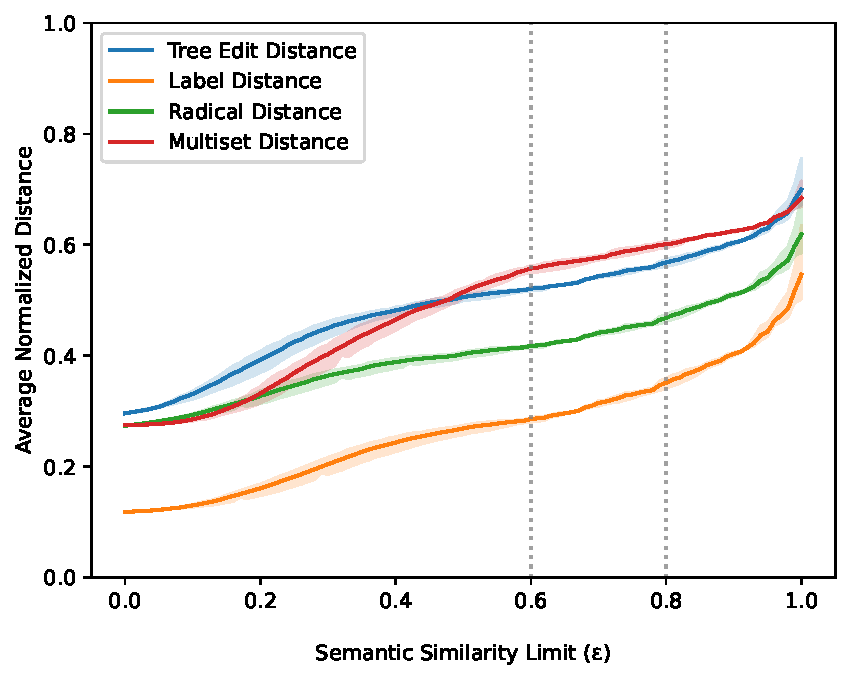
\includegraphics[width=\linewidth]{code/img/similaritylimits_at2_percentage.pdf}
    \caption{AT2 for semantic similarity limit ($\epsilon$) ranging from 0 to 1 with steps of 0.01}
    \label{fig:semsim-at2}
\end{figure}

In Figure~\ref{fig:semsim-at1-2}, we compare each AT1 to the AT2 generated by the same participant. We would expect all lines to be flat for all distance measures, as the only difference between AT1 and AT2 is additional nodes, which would be unaffected by $\epsilon$. This is the exact behavior we see for LD, TED, and RD. However, for MSD, we see a different behavior of riding distance with increasing $\epsilon$. This is cause by multiset semantics being generated from the leaf nodes only, which means that additional nodes (and especially additional leaf nodes) fundamentally change the multiset semantics. This behavior is unintuitive, and suggests that MSD may be unsuitable as an intuitive distance measure.



\begin{figure}
    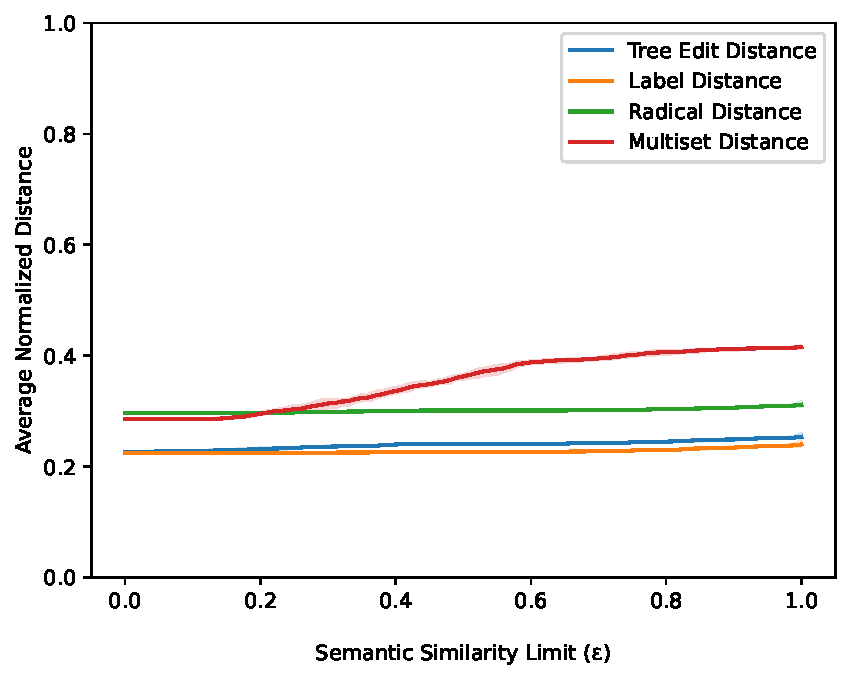
\includegraphics[width=\linewidth]{code/img/similaritylimits_at1-2_percentage.pdf}
    \caption{The comparison of AT1 and AT2 for semantic similarity limit ($\epsilon$) ranging from 0 to 1 with steps of 0.01}
    \label{fig:semsim-at1-2}
\end{figure}

In Figure~\ref{fig:semsim-at2}, we compare all AT2s together and generate an average distance, similar to what was does for Figure~\ref{fig:semsim-at1}. We expect the distance measures to behave similarly, as if each distance measures is fundamentally measuring the same thing, then the average across 38 different ATs should cause the behavior to normalize. We see this for LD, TED, and RD, where the distance changing at roughly the same rate with increasing $\epsilon$. However, for MSD, we see a pattern of behavior that does not match the other distance measures. This suggests that MSD is fundamentally not measuring the distance between attack trees, but something else. This is further evidence that MSD is not a valid measure of distance between attack trees.

\subsubsection{Comparison of operations}

One means of comparison across the different distance calculation is in how they differ by operation. As discussed in Section~\ref{ssec:ted}, we compare different modification ``operations'', which describe how one tree differs to another. In tree edit distance, this is the sequence of steps taken to modify one tree into another. In the other distance calculations, we can simulate these operations. Unlike tree edit distance, these operations will not necessarily yield a perfectly equivalent tree after modification; however, by counting these ``operations'' per different similarity limit ($\epsilon$) described in Section~\ref{sssec:threshold-problem}, we can better compare how the different distance calculations arrive at their final distance calculation.

We can see this comparison in Figure~\ref{fig:operations}, the distribution of operations for the different distance measures. We can see that for LD, RD, and TED, the distribution of operations is relatively consistent across the different similarity limits ($\epsilon$). However, for MSD, we see a different behavior. For MSD, the distribution of operations differs fairly significantly, which is further evidence of the lack of validity of MSD.

\begin{figure*}
\centering
\resizebox{\linewidth}{!}{
\begin{tabular}{lcccc}
Distance & Label Distance & Tree Edit Distance & Radical Distance & Multiset Distance \\
AT1 & 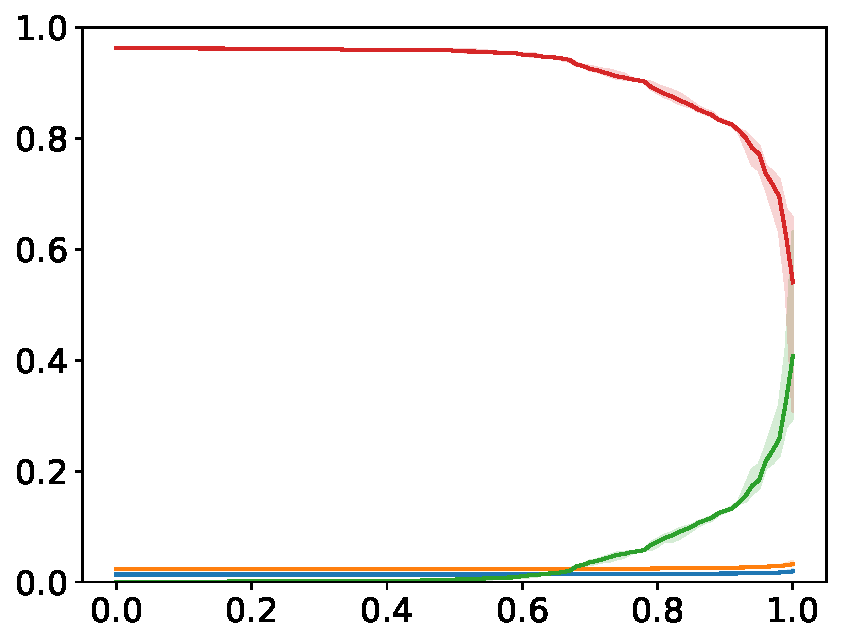
\includegraphics[width=.25\linewidth]{code/img/operation_count_ld_AT1.pdf} & 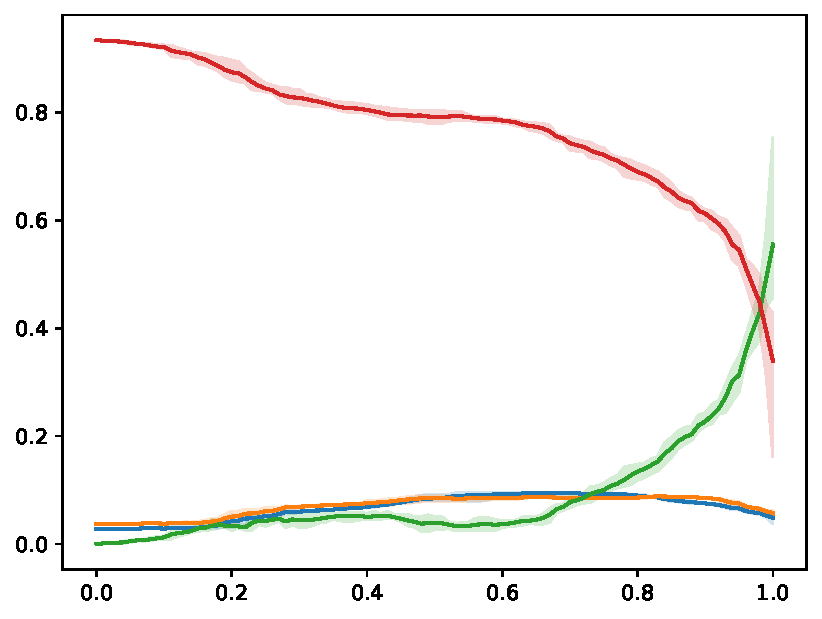
\includegraphics[width=.25\linewidth]{code/img/operation_count_zss_AT1.pdf} & 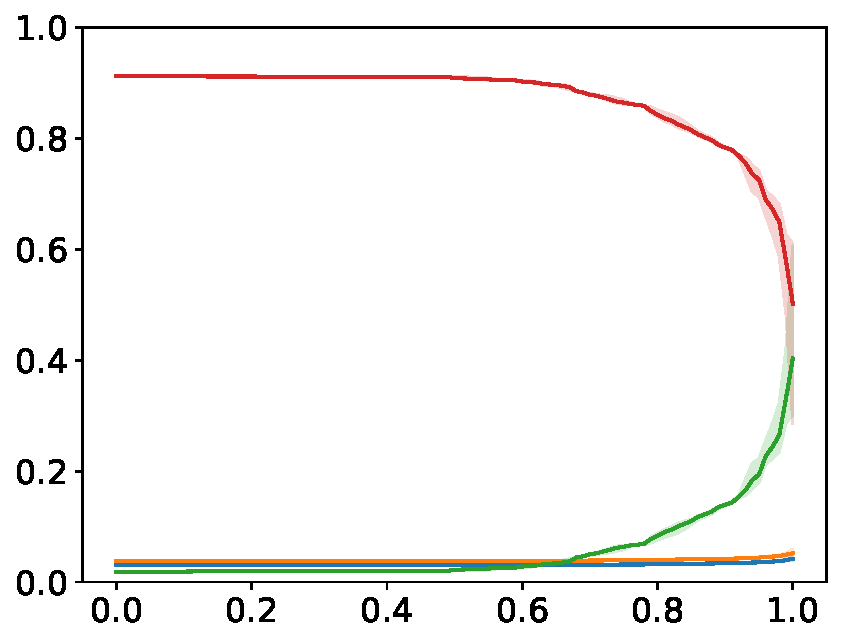
\includegraphics[width=.25\linewidth]{code/img/operation_count_rrd_AT1.pdf} & 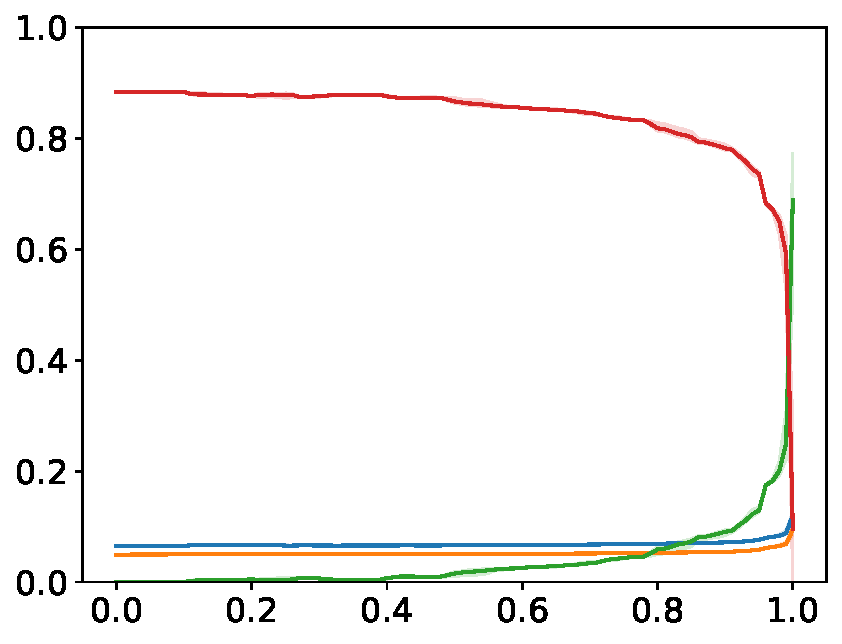
\includegraphics[width=.25\linewidth]{code/img/operation_count_ms_AT1.pdf} \\
AT1 vs AT2 & 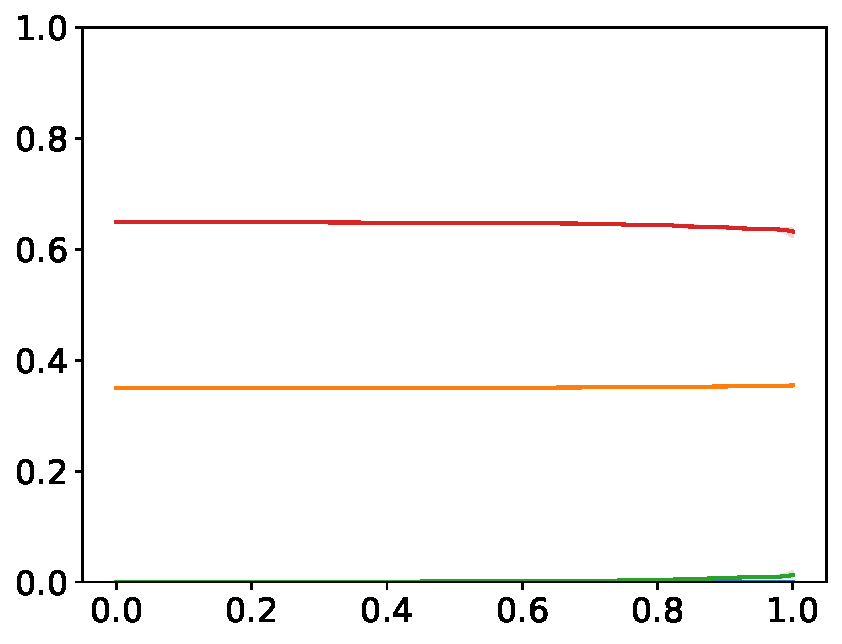
\includegraphics[width=.25\linewidth]{code/img/operation_count_ld_AT1-2.pdf} & 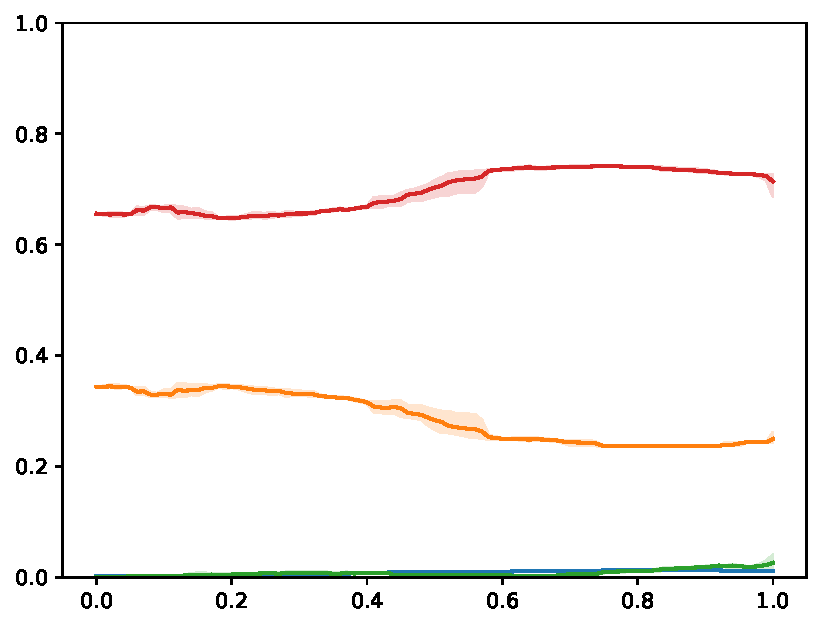
\includegraphics[width=.25\linewidth]{code/img/operation_count_zss_AT1-2.pdf} & 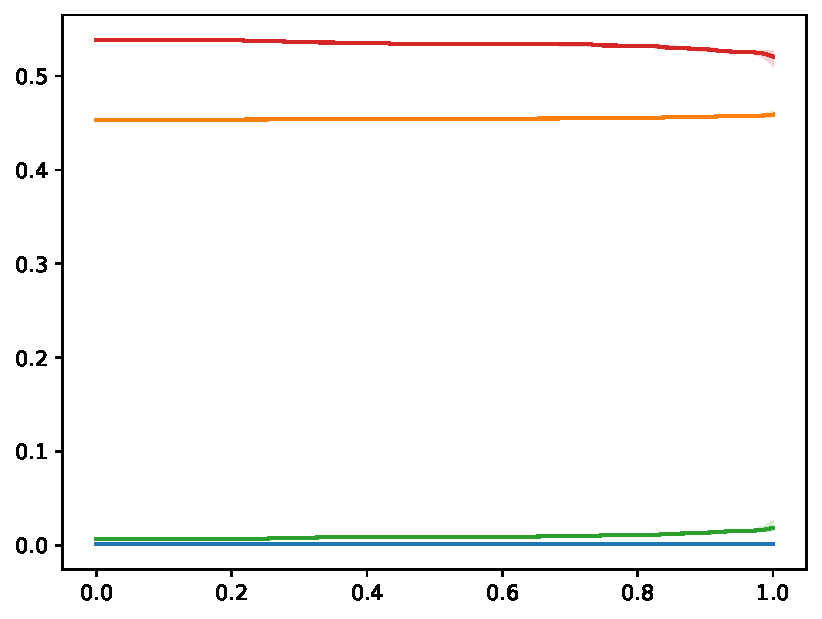
\includegraphics[width=.25\linewidth]{code/img/operation_count_rrd_AT1-2.pdf} & 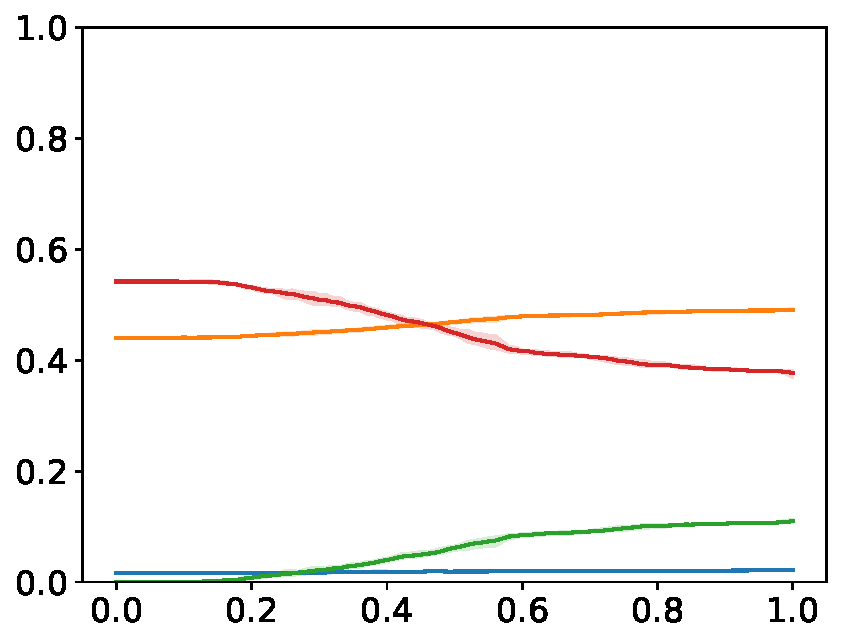
\includegraphics[width=.25\linewidth]{code/img/operation_count_ms_AT1-2.pdf} \\
AT2 & 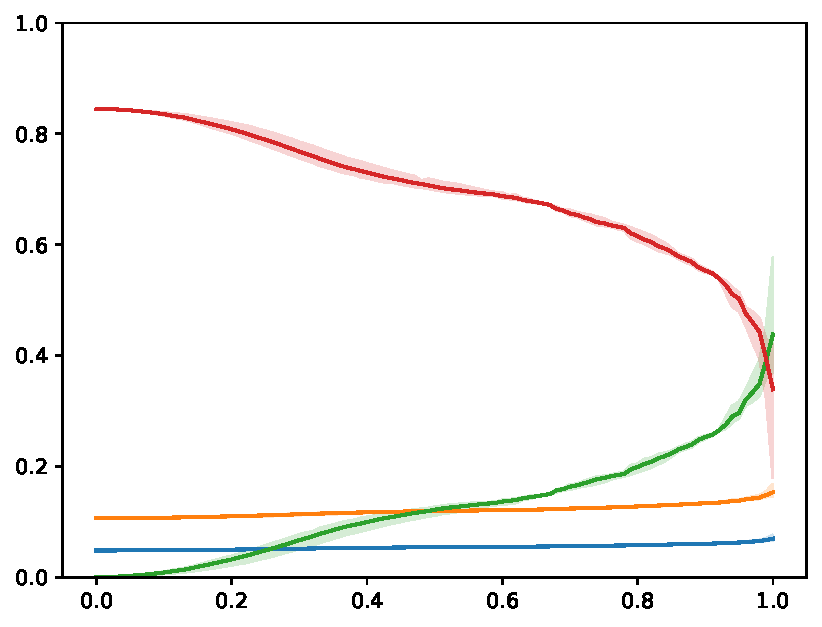
\includegraphics[width=.25\linewidth]{code/img/operation_count_ld_AT2.pdf} & 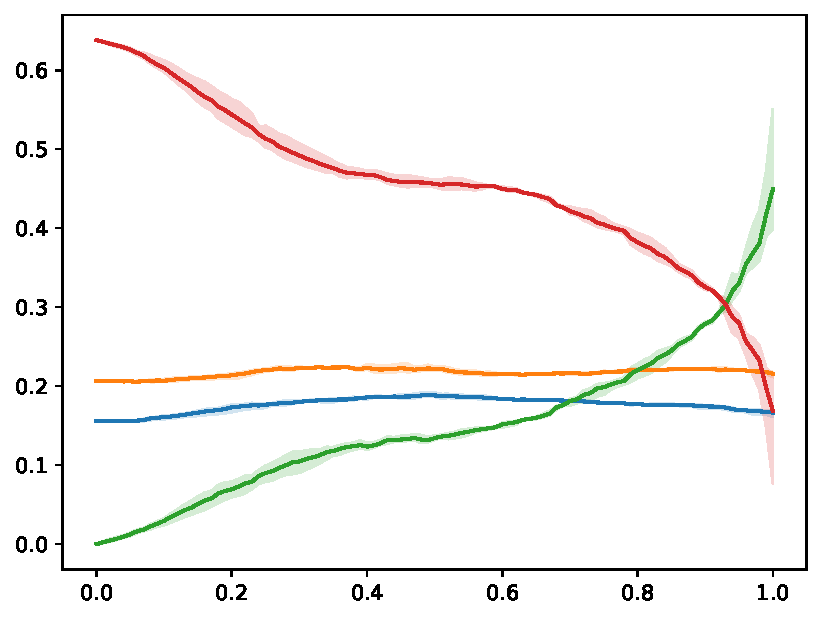
\includegraphics[width=.25\linewidth]{code/img/operation_count_zss_AT2.pdf} & 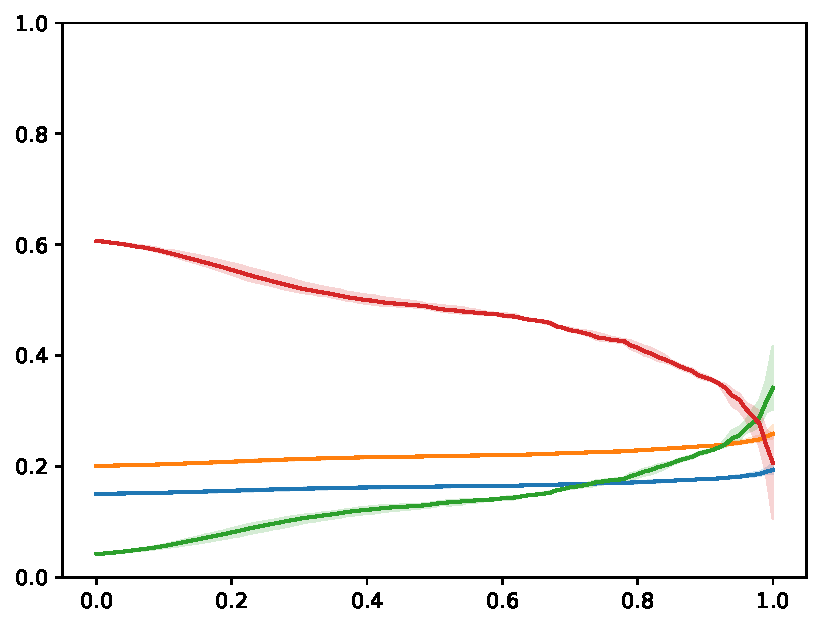
\includegraphics[width=.25\linewidth]{code/img/operation_count_rrd_AT2.pdf} & 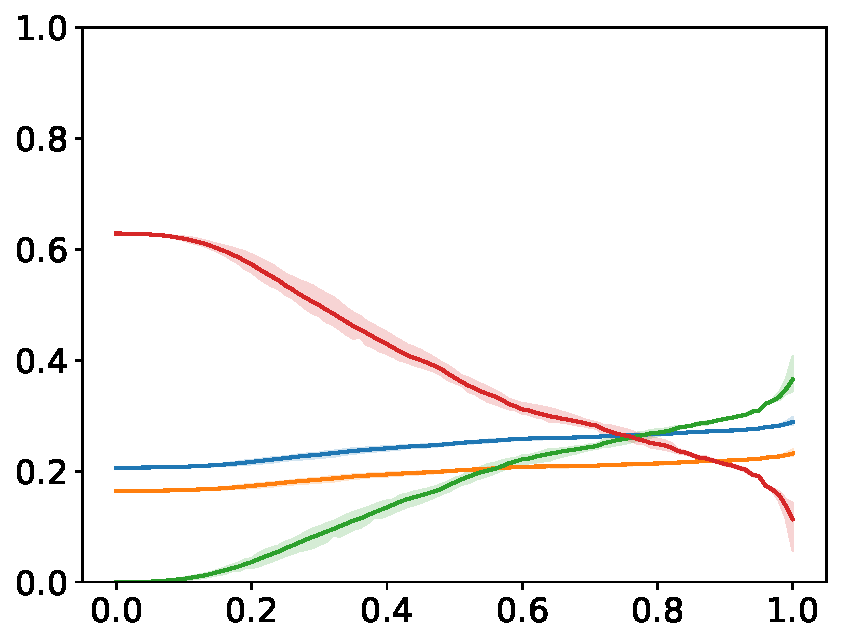
\includegraphics[width=.25\linewidth]{code/img/operation_count_ms_AT2.pdf}
\end{tabular}
}
\caption{Plots showing each type of modification operation as a percentage of the total number of operations for increasing similarity limit $\epsilon$. {\color{color1} \textbf{Blue}} indicates a removal operation. {\color{color2} \textbf{Orange}} indicates an addition operation. {\color{color3} \textbf{Green}} indicates a changing operation, and {\color{color4} \textbf{Red}} indicates a matching operation. }
\label{fig:operations}
\end{figure*}






\subsection{Basic Transformation Examples (BTEs)}
\label{ssec:results-examples}

\newcommand{\CERow}[9]{#1 & #2 & #3 & #4 & #5 & #7 & #8 & #9}
\newcommand{\WSDFootOne}{2}
\newcommand{\WSDFootTwo}{$\alpha_1$}
\newcommand{\WSDFootThree}{$\alpha_2$}
\newcommand{\WSDFootFour}{$\alpha_3$}
\begin{table*}[t]
\centering
\begin{tabular}{lc:cccc:ccc}
\toprule
\multicolumn{1}{c}{\multirow{2}{*}{\shortstack[l]{Basic Transformation\\Example (BTE)}}} &
\multicolumn{1}{c}{\multirow[c]{2}{*}{\shortstack{Intuitive\\answer}}}
&\multirow[c]{2}{*}{\shortstack{Label\\Distance} }
&\multirow[c]{2}{*}{\shortstack{Tree Edit\\Distance}}
&\multirow[c]{2}{*}{\shortstack{Radical\\Distance}}
&\multicolumn{1}{c}{\multirow[c]{2}{*}{\shortstack
        {Multiset\\Distance}}}
&\multicolumn{3}{c}{Weighted Sum Distance}
\\
% &\CERow{}{}{}{}{}{$[0.5, 0.25, 0.25, 0]$}{$[0.55, 0, 0.3, 0.15]$}{$[0.5, 0.5, 0, 0]$}{$[0.5, 0.15, 0.35, 0]$}
&\CERow{\multicolumn{1}{c}{}}{}{}{}{\multicolumn{1}{c}{}}{\WSDFootOne}{\WSDFootTwo}{\WSDFootThree}{\WSDFootFour}
\\
\midrule
Order Reversed &\CERow{0}{0}{7}{0}{0}{1.75}{0}{3.5}{1.05} \\
%\hdashline
Refinement Switch &\CERow{ 1}{0}{1}{1}{3}{0.5}{0.75}{0.5}{0.5} \\
Extra Intermediate &\CERow{ 1}{1}{1}{1}{0}{1}{0.85}{1}{1}  \\
Missing Intermediate &\CERow{ 1}{1}{1}{4}{0}{1.75}{1.75}{1}{2.05} \\
Extra Leaf &\CERow{ 1}{1}{1}{1}{1}{1}{1}{1}{1}  \\
Missing Leaf &\CERow{ 1}{1}{1}{1}{1}{1}{1}{1}{1}  \\
Changed Root &\CERow{ 1}{1}{1}{1}{0}{1}{.85}{1}{1}  \\
Changed Intermediate&\CERow{1}{1}{1}{1}{0}{1}{0.85}{1}{1}  \\
Changed Leaf &\CERow{ 1}{1}{1}{1}{1}{1}{1}{1}{1}  \\
Move Adjacent &\CERow{ 1}{0}{2}{2}{3}{1}{1.05}{1}{1}  \\
Move Up &\CERow{ 1}{0}{2}{2}{0}{1}{0.6}{1}{1}  \\
Move Down &\CERow{ 1}{0}{2}{3}{1}{1.25}{1.05}{1}{1.35} \\
\bottomrule
    \end{tabular}
\caption{The distances provided by each of the distance measurements. The intuitive distance for each of these BTEs is provided in column 1\\
\footnotesize
% \WSDFootOne: We use a weighted value of $\alpha = [.5, .25, .25, 0]$\\
\WSDFootTwo: We use a weighted value of $\alpha = [0.55, 0, 0.30, 0.15]$\\
\WSDFootThree: We use a weighted value of $\alpha = [0.5, 0.5, 0, 0]$\\
\WSDFootFour: We use a weighted value of $\alpha = [0.5, 0.15, 0.35, 0]$\\
\normalsize}
\label{tab:counterexamples}
\end{table*}

\newcommand{\WSDWidth}{.45\linewidth}
\begin{figure*}[t]
    \centering
    \begin{subfigure}[b]{\WSDWidth}
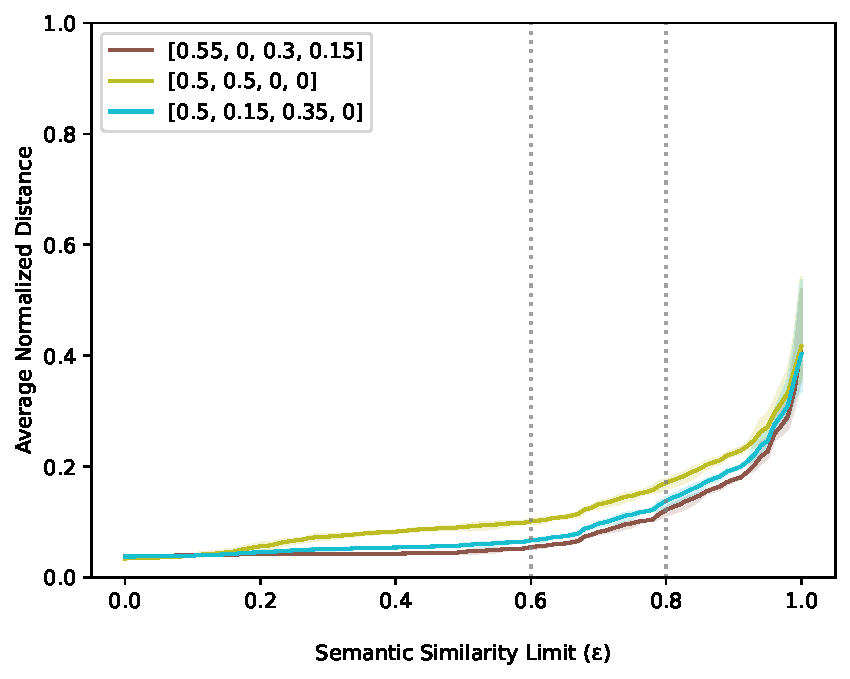
\includegraphics[width=\linewidth]{code/img/wsd-at1-3alphas-no-background.pdf}
        \caption{WSD on AT1}
        \label{fig:wsd-at1}
    \end{subfigure}
    \begin{subfigure}[b]{\WSDWidth}
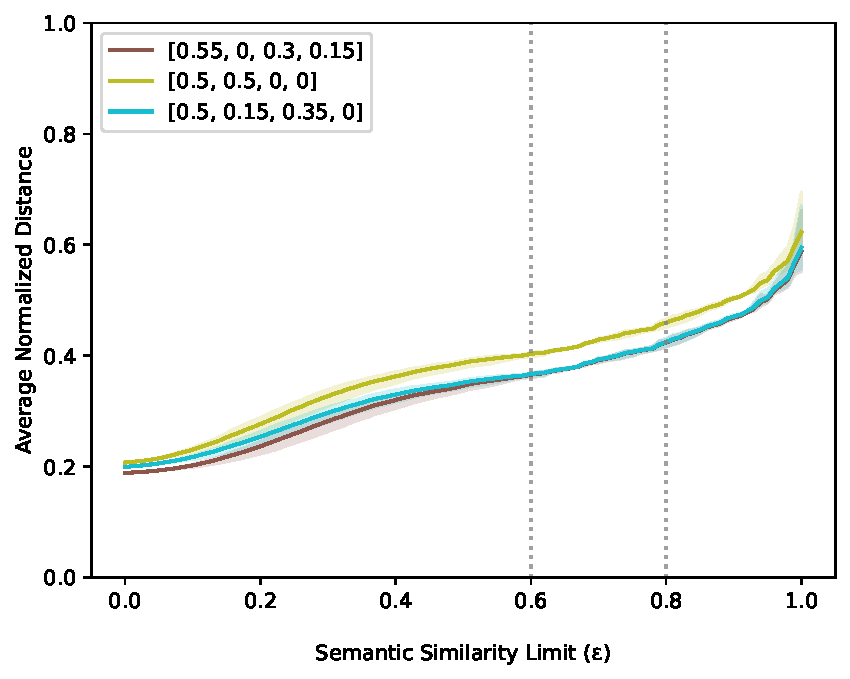
\includegraphics[width=\linewidth]{code/img/wsd-at2-3alphas-no-background.pdf}
        \caption{WSD on AT2}
        \label{fig:wsd-at2}
    \end{subfigure}
    \caption{WSD on AT1 and AT2 using the optimal $\alpha$ value established in Section~\ref{ssec:results-alpha}}
    \label{fig:wsd}
\end{figure*}

As enumerated in Section~\ref{ssec:methodology-examples}, we have 12 examples of various basic transformation examples (BTEs) that could occur between attack trees. These are meant to assess if each of our distance measures is able to represent these changes in a manner we would consider intuitive. The absolute distance for each distance measure for each example is provided in Table~\ref{tab:counterexamples}. Fundamentally, all changes between two attack can be described as a series of transformations described by our BTEs.

In Table~\ref{tab:counterexamples}, we describe an ``intuitive answer''. This is what we believe a practitioner would describe as the distance between the given BTEs and the base attack tree, shown in Figure~\ref{sfig:base}. The intuitive answer is the number of ``operations'' that would be required to convert the base attack tree into the BTE.

We can see that TED nearly perfectly follows our intuition, with the major exception of nodes that are not in order. In this example, the tree edit distance marks that all nodes need to be changed as it is unable to match any nodes. This behavior is to be expected as TED is meant to be run on an ordered tree. Algorithms to calculate unordered TED exist, however they are incompatible with our usage of semantic similarity. Each of these algorithms makes assumptions about equality, and these assumptions cannot be made in our case.

Label distance behaves exactly as expected, it perfectly matches the intuitive answer for all examples in which a label is changed, added or removed. It then does not match the intuition for any example in which the labels all remain the same but the structure is changed in some way.

Radical distance nearly matches the intuitive answer except for a few specific situations. In the example of a missing intermediate node, radical distance considers this as needing to remove threes nodes (the leaf nodes in the base attack tree and the intermediate) and then re-adding the two leaf nodes. This is caused as the radicals are mapped between the two trees by their roots, which means that radical distance has no mechanism to recognize that the two child nodes of one radical best suit another radical. This is potentially addressable with a post processing step checking for mappings in which the same label is added and removed. For the example of moving a node down, this creates a new radical, which causes radical distance to add an extra value of one. Additionally, if we applied a post processing step of removing additional and removal operations of identical labels, then all of the movement BTEs would have resulted in 0 distance (as all examples consist of removing and adding the same node). As such, this post processing step may result in unexpected behavior.

Finally, MSD behaves in ways that are not at all intuitive. First, because of the construction of multisets, only the labels of leaf nodes are considered in the calculation. Some structure of the original tree exists in how the multisets are constructed, but reconstruction of the original tree is not possible \cite{mauw_foundations_2006}. Any modification that only applied to intermediate nodes or the root node will not be represented by multiset representations of attack trees, which likewise results in a distance of 0. For changes that affect leaf nodes, multiset semantics seem to over-represent the distance. In the 12 BTEs we created, multiset semantics only provided the intuitive distance in 4 cases.







\subsection{Determining optimal $\alpha$ for Weighted Sum Distance}
\label{ssec:results-alpha}

% Looking at Table~\ref{tab:counterexamples}, we find that LD, TED, and RD all fail to match our intuitive understanding of distance on four BTEs. However, as discussed, they all fail on different BTEs. We can thus weight $\alpha_1$, $\alpha_2$, and $\alpha_3$ according to their performance. Additionally, we can see that MSD fails to match our intuitive understanding of distance on 7 BTEs. As such, we can weight $\alpha_4$ as 0. We find an optimal $\alpha$ value of $[0.5, 0.25, 0.25, 0]$. This also fails for four of our BTEs, but by a smaller margin than either LD, TED, or RD individually. For this $\alpha$, WSD is optimal. We use this $\alpha$ value for the WSD values in this paper.

Looking at Table~\ref{tab:counterexamples}, we find that LD, TED, and RD all fail to match our intuitive understanding of distance on four BTEs. However, they all fail on different BTEs. MSD fails to match our intuition on seven of our BTEs.

Using our intuitive understanding of the distance values for our BTEs, we can develop three potential $\alpha$ values for WSD. The first, $\alpha_1$, is aimed at reducing the difference between our intuitive understanding of distance for each BTE and the distance calculated by WSD. We find this value to be $\alpha_1=[0.55, 0, 0.3, 0.15]$, and it results in a total deviation of 1.95 from our intuition spread across a total of eight incorrect BTEs.

The second, $\alpha_2$, is aimed at reducing the number of BTEs that are incorrect. We find this value to be $\alpha_2=[0.5,0.5,0,0]$, and it results in a total deviation of 4 from our intuition spread across a total of two incorrect BTEs. Finally, we calculate $\alpha_3$ which is intended to be an optimal value between these two extremes, opimizing for both total incorrect BTEs and total deviation from our intuition. We find this value to be $\alpha_3=[0.5, 0.15, 0.35, 0]$, and it results in a total deviation of 2.95 from our intuition spread across a total of four incorrect BTEs.

\newcommand{\ReqFootOne}{3}
\newcommand{\ReqFootTwo}{4}
\newcommand{\ReqFootThree}{5}
\newcommand{\ReqTableRow}[9]{#1 & #2 & #3 & #4 & #5 & #6 & #7 & #8 & #9}
\begin{table*}[t!]
    \centering
    \resizebox{\linewidth}{!}{%
        \begin{tabular}{@{}lcccc:ccc:cc@{}}
            \toprule
            \shortstack{\textbf{Distance}                                                                                                                                                                                                        \\\textbf{Measure}\\\text{ }}
                         & \shortstack{\req{1}                                                                                                                                                                                                   \\\textbf{Metric}\\\text{ }}
                         & \shortstack{\req{2}                                                                                                                                                                                                   \\\textbf{Position}\\\text{ }}
                         & \shortstack{\req{3}                                                                                                                                                                                                   \\\textbf{Refinements}\\\text{ }}
                         & \shortstack{\req{4}                                                                                                                                                                                                   \\\textbf{Labels}\\\text{ }}
                         & \shortstack{\req{5}                                                                                                                                                                                                   \\\textbf{Unordered}\\\text{ }}
                         & \shortstack{\req{6}                                                                                                                                                                                                   \\\textbf{Unfiltered}\\\text{ }}
                         & \shortstack{\req{7}                                                                                                                                                                                                   \\\textbf{Intuitive}\\\text{ }}
                         & \shortstack{\req{8}                                                                                                                                                                                                   \\\textbf{Theoretically}\\\textbf{Valid}}
                         & \shortstack{\req{9}                                                                                                                                                                                                   \\\textbf{Experimentally}\\\textbf{Valid}}
            \\ \midrule
            %\textbf{Statistics}       & \Negate                & \Confirm\footnotemark[1]          & \Negate \footnotemark[2]        & \Confirm          &\Confirm   & \Negate                 & \Confirm           & \Negate                   & \Negate\footnotemark[2]                    \\
            \textbf{TED} & \Confirm            & \Confirm & \Confirm                           & \Confirm                           & \Negate  & \Confirm & \Confirm & \Partial\footnotemark[\ReqFootOne] & \Confirm                             \\
            \textbf{LD}  & \Confirm            & \Negate  & \Negate                            & \Confirm                           & \Confirm & \Confirm & \Confirm & \Partial\footnotemark[\ReqFootOne] & \Confirm                             \\
            \textbf{RD}  & \Confirm            & \Confirm & \Confirm                           & \Confirm                           & \Confirm & \Confirm & \Confirm & \Partial\footnotemark[\ReqFootOne] & \Confirm                             \\
            \textbf{MSD} & \Confirm            & \Negate  & \Partial\footnotemark[\ReqFootTwo] & \Partial\footnotemark[\ReqFootTwo] & \Confirm & \Confirm & \Negate  & \Partial\footnotemark[\ReqFootOne] & \Partial\footnotemark[\ReqFootThree] \\ \bottomrule
        \end{tabular}
    }
    \caption{A comparison of the different distance measures and their suitability w.r.t. the requirements defined in Section~\ref{ssec:requirements}\\
        \footnotesize
        \ReqFootOne: All distance measures failed on at least on of our BTEs\\
        \ReqFootTwo: MSD does not include all nodes, but does contain some information about refinements for the nodes that are included\\
        \ReqFootThree: MSD exhibits behavior on the experimental dataset that does not align with our expectations. As such, the experimental validity is inconclusive.
        \normalsize}
    \label{tab:requirmeent-suitability}
\end{table*}


Our three optimal $\alpha$ values are shown on Table~\ref{tab:counterexamples}. Additionally, these three values are shown on AT1 and AT2 with varying $\epsilon$ in Figures~\ref{fig:wsd-at1}~and~\ref{fig:wsd-at2}. We can see the variations between the different optimal values of $\alpha$ are relatively minute. Further, we can see the variations caused by the different models for each WSD line to be smaller than for the other distances, shown in Figures~\ref{fig:semsim-at1},~\ref{fig:semsim-at2}~and~\ref{fig:semsim-at1-2}, suggesting that WSD may be an ideal way to reduce other sources of variation between distance. Overall, we see consistent behavior with WSD for well chosen $\alpha$, that is in line with our expectations described in Section~\ref{ssec:method-analysis}; most importantly, that for Figure~\ref{fig:wsd-at2}, the values are consistent across the different distance measures, indicating a reliable and consistent distance measure.










% \subsection{Measuring $\gamma(\Delta)$}

% \NS{Operations plot}

% \subsection{Finding optimal $\epsilon$}

% In Figure~\ref{img:similaritylimits}, we can see the effect of rising semantic similarity limit ($\epsilon$) on the average distance between each of attack tree 1 ($n=38$). Additionally, we can see the normalized Levenshtein distance plotted against the same semantic similarity limits. Finally, we can see the traditional Zhang and Shasha edit distance (based on string equivalence), which is unaffected by a similarity limit.

% \begin{figure}
% 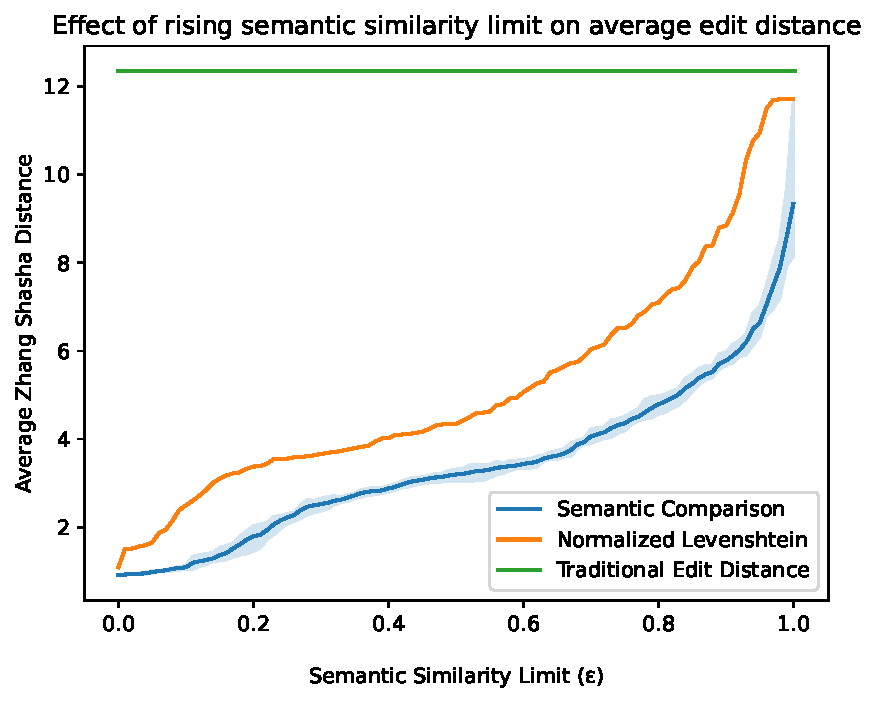
\includegraphics[width=\linewidth]{code/img/similaritylimits2.pdf}
% \caption{The average distance between the 38 experimental ATs per semantic similarity limit}
% \label{img:similaritylimits}
% \end{figure}

% \NS{Operations plot}


% \section{Effect of node flipping}

% \NS{plot showing average distance between 38 ATs with and without node flipping}




% \newcommand{\CERow}[9]{#1 & #2 & #3 & #4 & #5 & #7 & #8 & #9}
% \newcommand{\WSDFootOne}{2}
% \newcommand{\WSDFootTwo}{2}
% \newcommand{\WSDFootThree}{3}
% \newcommand{\WSDFootFour}{4}
% \begin{table*}[t]
% \centering
% \begin{tabular}{lccccc:ccc}
% \toprule

% \shortstack[l]{Basic Transformation\\Example (BTE)} & \CERow{\shortstack{Intuitive\\answer} }{ \shortstack{Label\\Distance} }{ \shortstack{Tree Edit\\Distance} }{ \shortstack{Radical\\Distance} }{ \multicolumn{1}{c}{\shortstack{Multiset\\Distance} }}{\multicolumn{1}{c}{\shortstack{Weight Sum\\Distance\footnotemark[\WSDFootOne]}}}{\multicolumn{1}{c}{\shortstack{Weight Sum\\Distance\footnotemark[\WSDFootTwo]}}}{\multicolumn{1}{c}{\shortstack{Weight Sum\\Distance\footnotemark[\WSDFootThree]}}}{\multicolumn{1}{c}{\shortstack{Weight Sum\\Distance\footnotemark[\WSDFootFour]}}}\\
% \midrule
% Order Reversed &\CERow{0}{0}{7}{0}{0}{1.75}{0}{3.5}{1.05} \\\hdashline
% Refinement Switch &\CERow{ 1}{0}{1}{1}{3}{0.5}{0.75}{0.5}{0.5} \\
% Extra Intermediate &\CERow{ 1}{1}{1}{1}{0}{1}{0.85}{1}{1}  \\
% Missing Intermediate &\CERow{ 1}{1}{1}{4}{0}{1.75}{1.75}{1}{2.05} \\
% Extra Leaf &\CERow{ 1}{1}{1}{1}{1}{1}{1}{1}{1}  \\
% Missing Leaf &\CERow{ 1}{1}{1}{1}{1}{1}{1}{1}{1}  \\
% Changed Root &\CERow{ 1}{1}{1}{1}{0}{1}{.85}{1}{1}  \\
% Changed Intermediate&\CERow{1}{1}{1}{1}{0}{1}{0.85}{1}{1}  \\
% Changed Leaf &\CERow{ 1}{1}{1}{1}{1}{1}{1}{1}{1}  \\
% Move Adjacent &\CERow{ 1}{0}{2}{2}{3}{1}{1.05}{1}{1}  \\
% Move Up &\CERow{ 1}{0}{2}{2}{0}{1}{0.6}{1}{1}  \\
% Move Down &\CERow{ 1}{0}{2}{3}{1}{1.25}{1.05}{1}{1.35} \\
% \bottomrule
%     \end{tabular}
% \caption{The distances provided by each of the distance measurements. The intuitive distance for each of these BTEs is provided in column 1\\
% \footnotesize
% % \WSDFootOne: We use a weighted value of $\alpha = [.5, .25, .25, 0]$\\
% \WSDFootTwo: We use a weighted value of $\alpha = [0.55, 0, 0.30, 0.15]$\\
% \WSDFootThree: We use a weighted value of $\alpha = [0.5, 0.5, 0, 0]$\\
% \WSDFootFour: We use a weighted value of $\alpha = [0.5, 0.15, 0.35, 0]$\\
% \normalsize}
% \label{tab:counterexamples}
% \end{table*}